\section{Qualitative Audit Samples}
\label{app:audit_samples}

This appendix presents 20 paired qualitative audit samples comparing \texttt{DetectorNX-G3-SNN} (left) and \texttt{DetectorNX-G3-CNN} (right) predictions on the ETraM validation set. Each row shows the same input scene, allowing direct visual comparison of detection behaviour between the two architectures. Samples are grouped by what they are intended to demonstrate, beginning with baseline-competence cases and progressing through the architectures' divergent behaviour, calibration evidence, and shared failure modes.

Within each rendered frame, the green solid box denotes the ground-truth annotation, the red dashed box denotes the model's prediction, and per-detection confidence scores are overlaid in red. The frame header records the validation-set sample index together with the prediction and ground-truth object counts.

\renewcommand{\arraystretch}{1.2}
\setlength{\tabcolsep}{4pt}

\begin{longtable}{@{}cc@{}}
\textbf{DetectorNX-G3-SNN} & \textbf{DetectorNX-G3-CNN} \\
\hline
\endfirsthead
\textbf{DetectorNX-G3-SNN} & \textbf{DetectorNX-G3-CNN} \\
\hline
\endhead
\hline
\multicolumn{2}{r}{\textit{continued on next page}} \\
\endfoot
\hline
\endlastfoot
%
% ============================================================
% 1. Single-Vehicle Successes
% ============================================================
\multicolumn{2}{@{}l@{}}{\rule{0pt}{4ex}\textbf{\large 1. Single-Vehicle Successes}} \\
\multicolumn{2}{@{}p{0.94\textwidth}@{}}{\itshape\small Baseline-competence cases. Both models tightly localise the ground-truth box at high confidence.} \\
\hline

\includegraphics[width=0.45\textwidth]{chapter_3/dnx_results/snn_audit/audit_sample_008.png} & 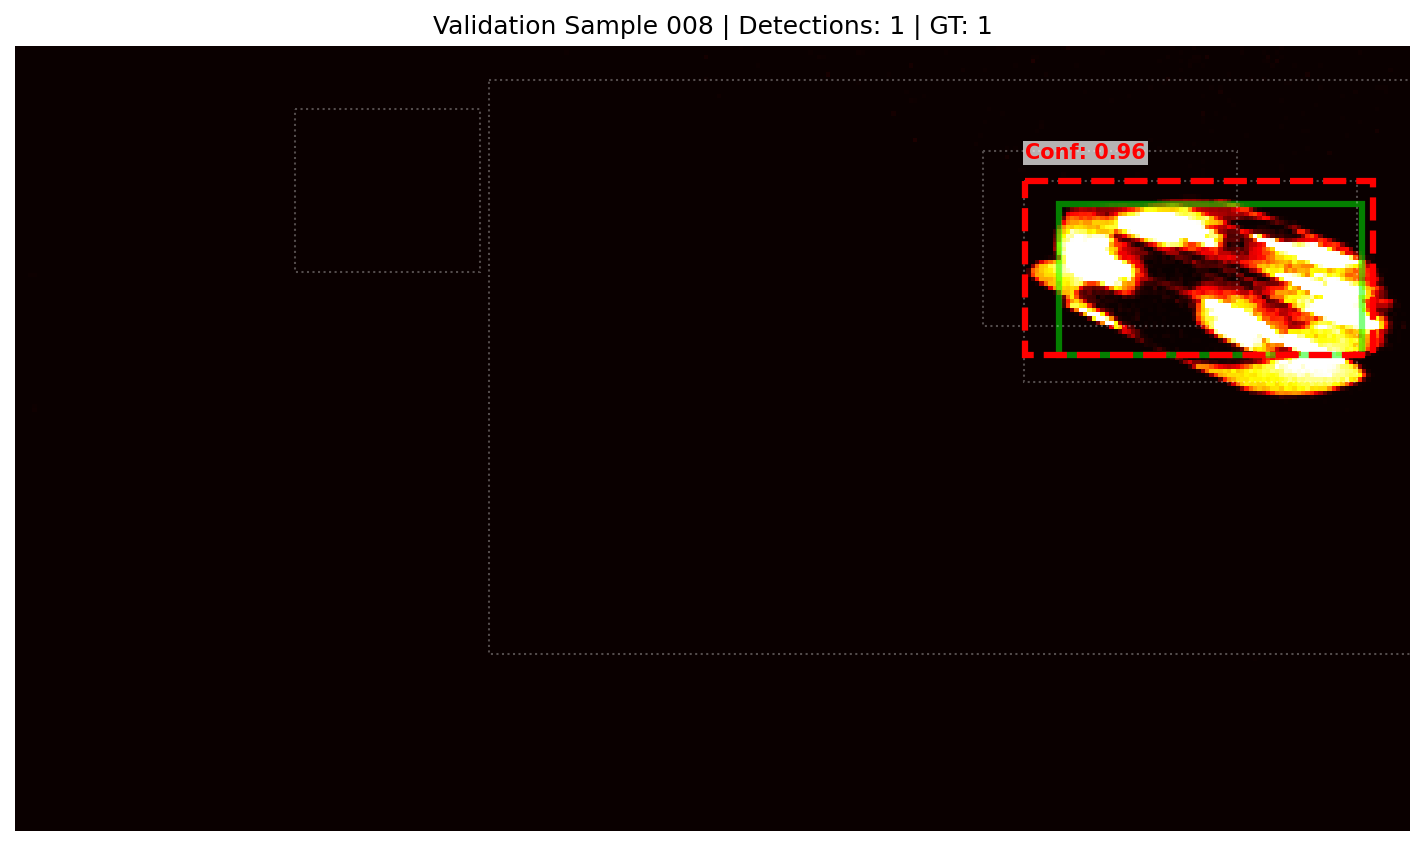
\includegraphics[width=0.45\textwidth]{chapter_3/dnx_results/cnn_audit/audit_sample_008.png} \\
\multicolumn{2}{@{}>{\centering\arraybackslash}p{0.92\textwidth}@{}}{\small\textit{Sample 008}} \\[0.5em]

\includegraphics[width=0.45\textwidth]{chapter_3/dnx_results/snn_audit/audit_sample_045.png} & 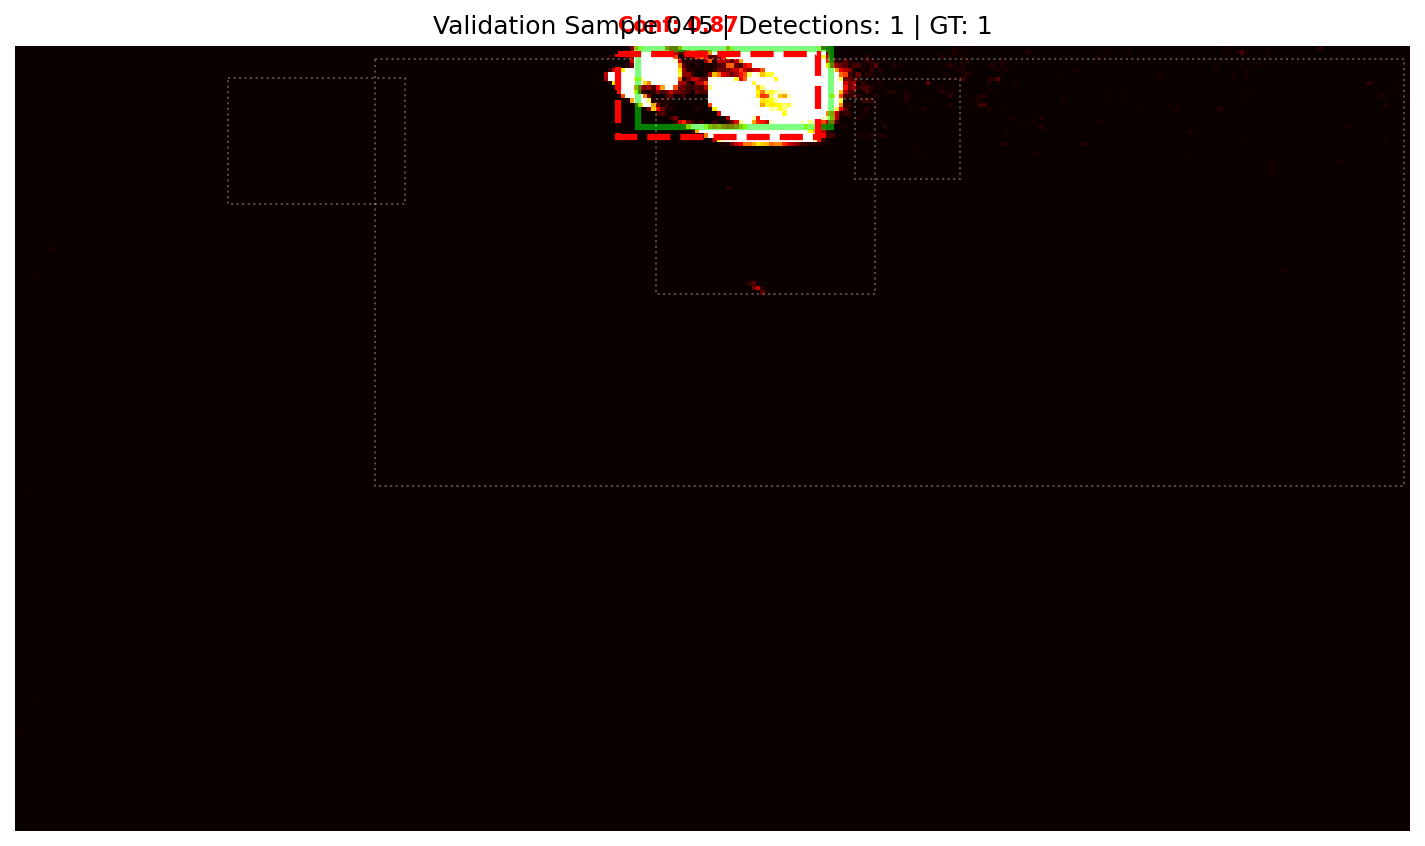
\includegraphics[width=0.45\textwidth]{chapter_3/dnx_results/cnn_audit/audit_sample_045.png} \\
\multicolumn{2}{@{}>{\centering\arraybackslash}p{0.92\textwidth}@{}}{\small\textit{Sample 045}} \\[0.5em]

% ============================================================
% 2. Multi-Vehicle Scenes (Both Models Correct)
% ============================================================
\multicolumn{2}{@{}l@{}}{\rule{0pt}{4ex}\textbf{\large 2. Multi-Vehicle Scenes — Both Models Correct}} \\
\multicolumn{2}{@{}p{0.94\textwidth}@{}}{\itshape\small Six two-vehicle scenes spanning different spatial layouts and event densities. The repeated competence here is intentional: parity is not a single lucky frame.} \\
\hline

\includegraphics[width=0.45\textwidth]{chapter_3/dnx_results/snn_audit/audit_sample_055.png} & 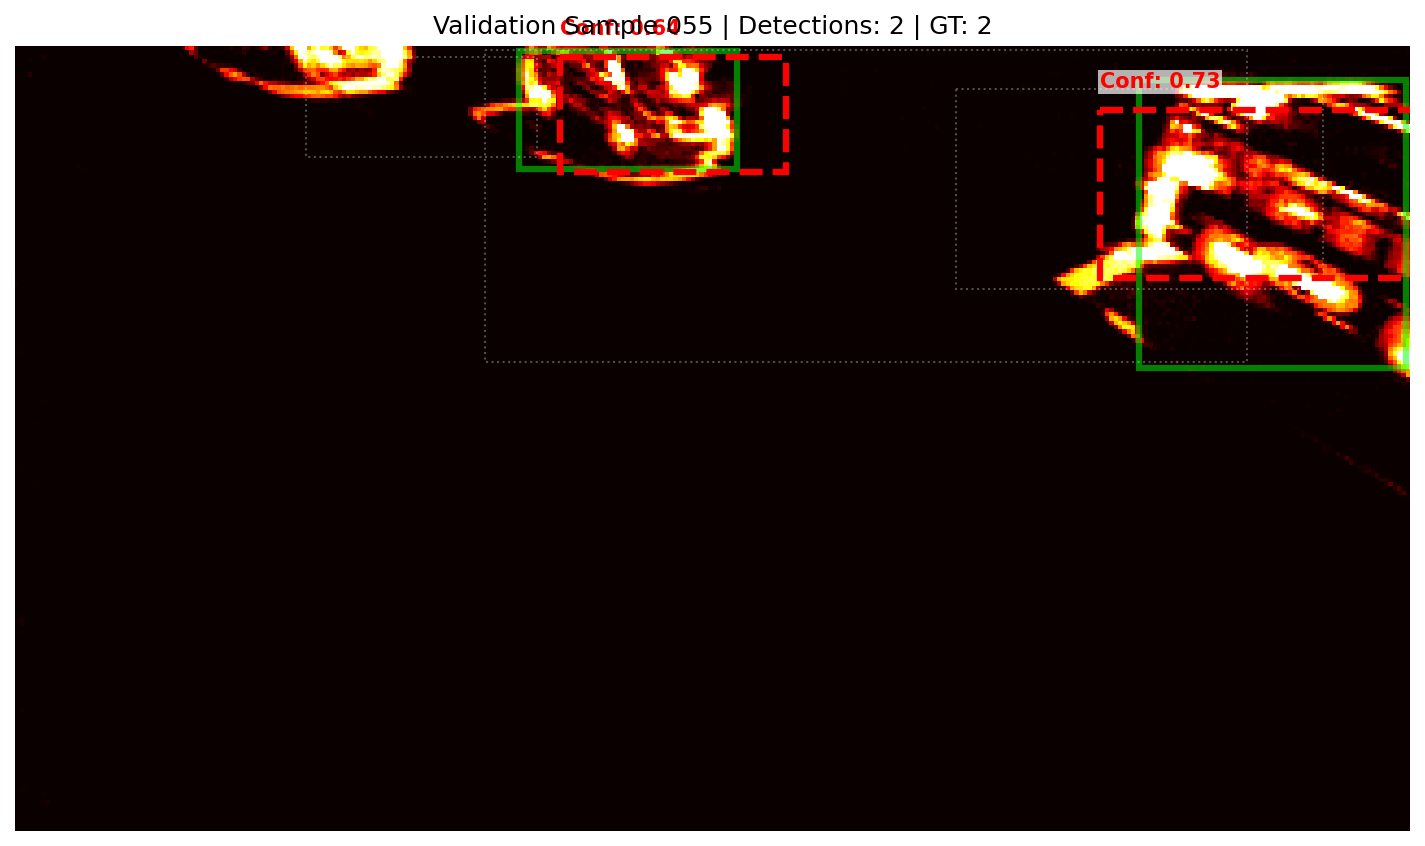
\includegraphics[width=0.45\textwidth]{chapter_3/dnx_results/cnn_audit/audit_sample_055.png} \\
\multicolumn{2}{@{}>{\centering\arraybackslash}p{0.92\textwidth}@{}}{\small\textit{Sample 055}} \\[0.5em]

\includegraphics[width=0.45\textwidth]{chapter_3/dnx_results/snn_audit/audit_sample_062.png} & 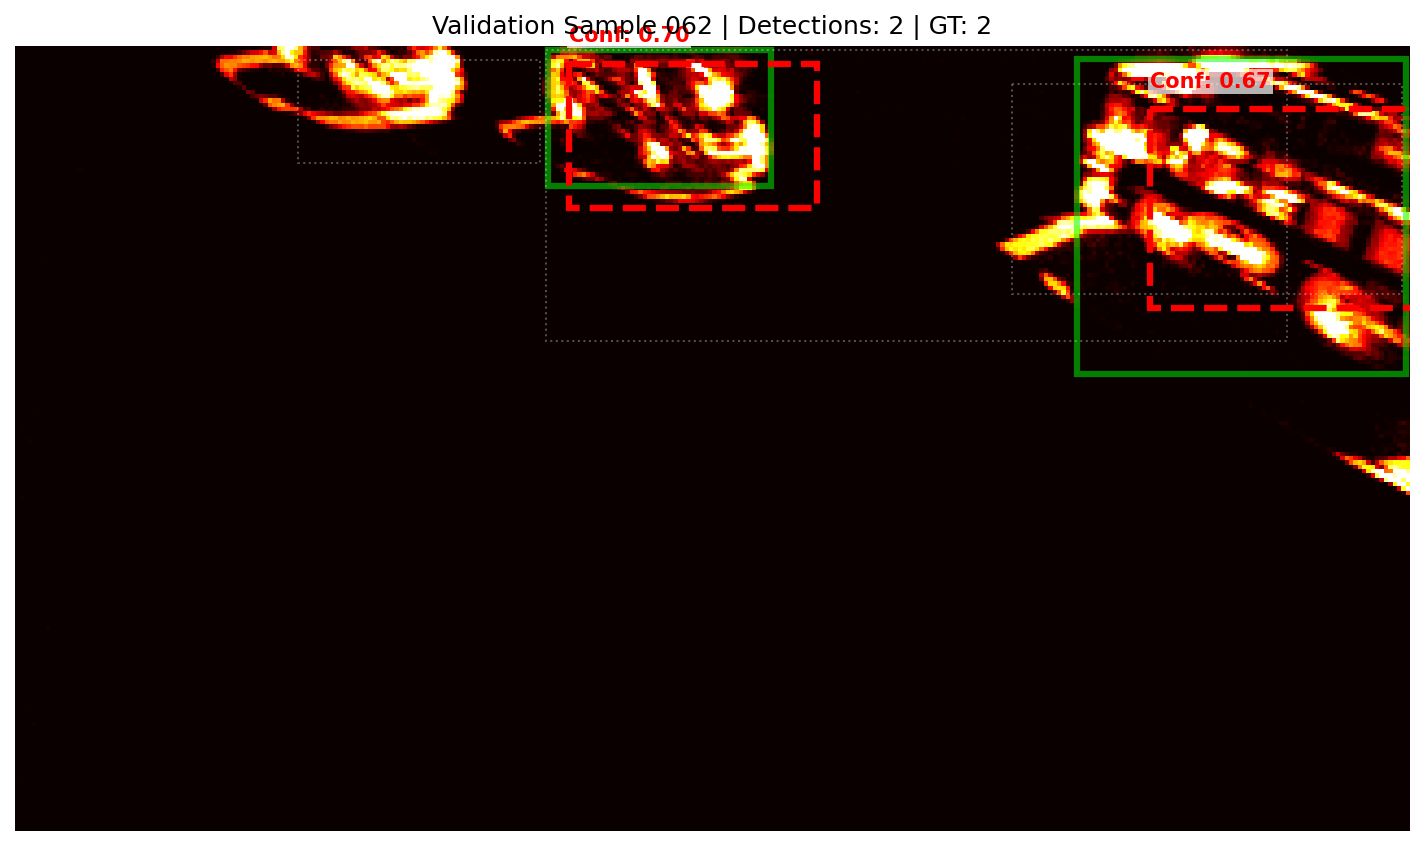
\includegraphics[width=0.45\textwidth]{chapter_3/dnx_results/cnn_audit/audit_sample_062.png} \\
\multicolumn{2}{@{}>{\centering\arraybackslash}p{0.92\textwidth}@{}}{\small\textit{Sample 062}} \\[0.5em]

\includegraphics[width=0.45\textwidth]{chapter_3/dnx_results/snn_audit/audit_sample_072.png} & 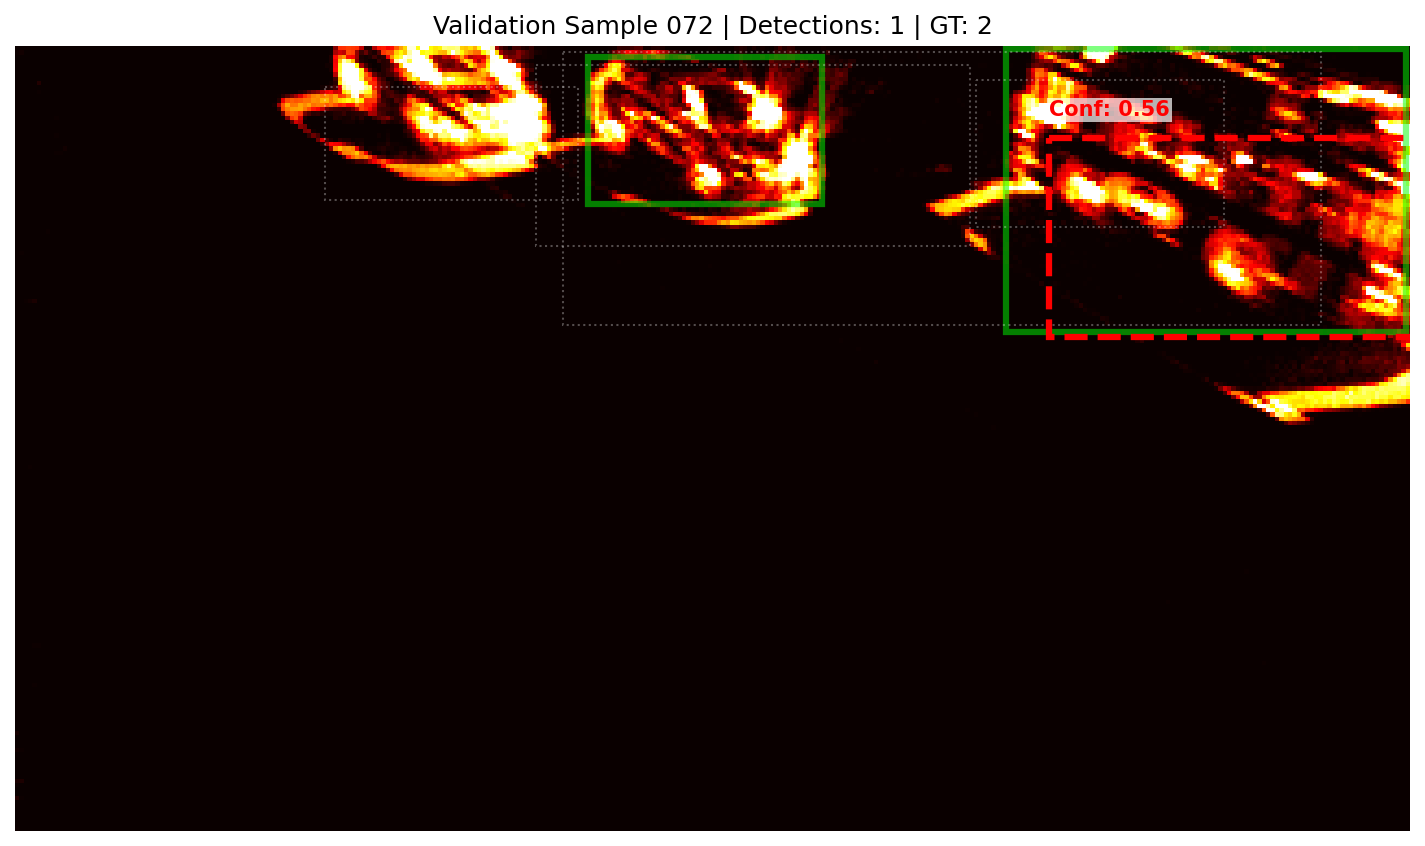
\includegraphics[width=0.45\textwidth]{chapter_3/dnx_results/cnn_audit/audit_sample_072.png} \\
\multicolumn{2}{@{}>{\centering\arraybackslash}p{0.92\textwidth}@{}}{\small\textit{Sample 072}} \\[0.5em]

\includegraphics[width=0.45\textwidth]{chapter_3/dnx_results/snn_audit/audit_sample_145.png} & 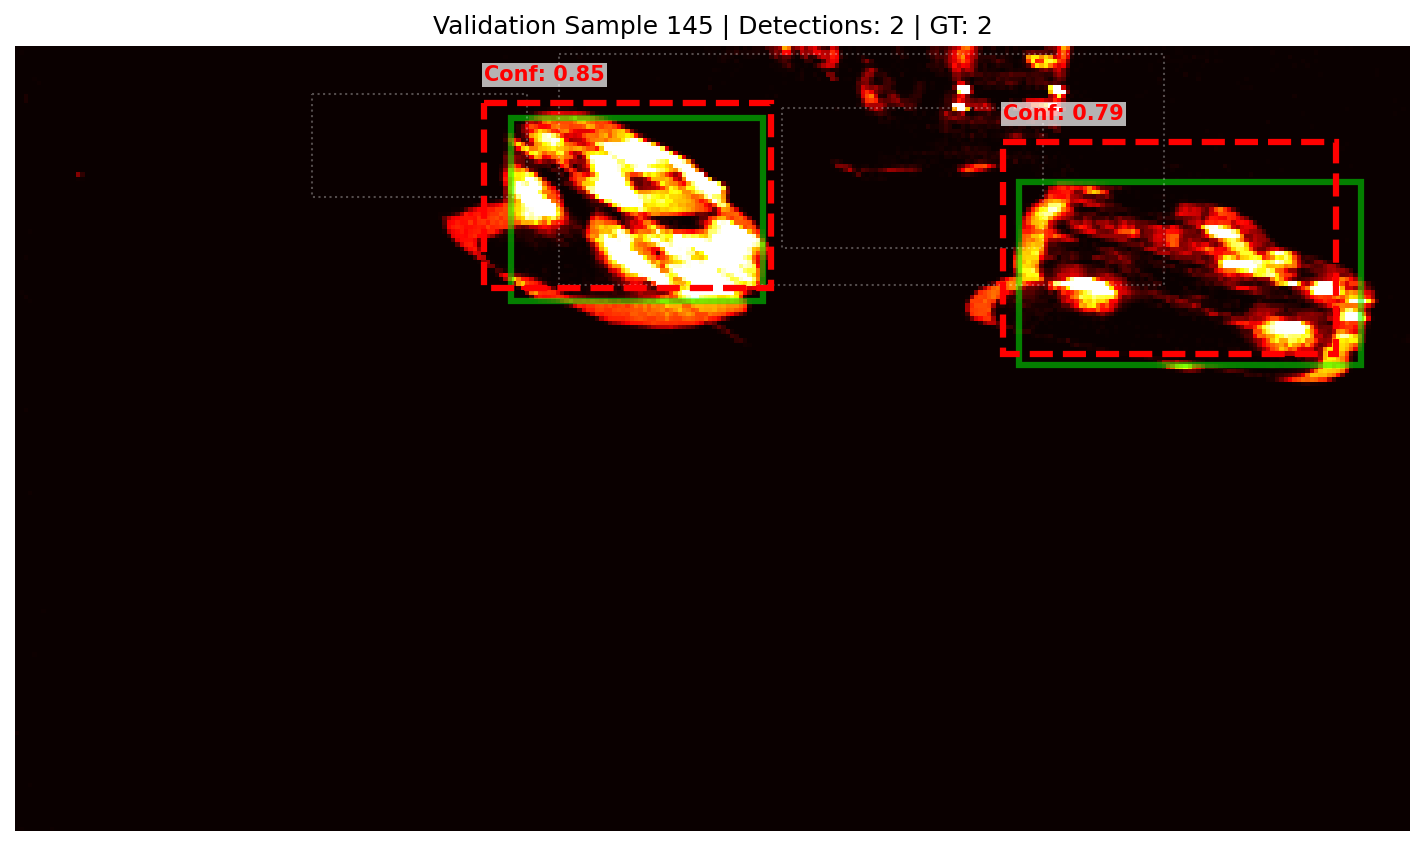
\includegraphics[width=0.45\textwidth]{chapter_3/dnx_results/cnn_audit/audit_sample_145.png} \\
\multicolumn{2}{@{}>{\centering\arraybackslash}p{0.92\textwidth}@{}}{\small\textit{Sample 145}} \\[0.5em]

\includegraphics[width=0.45\textwidth]{chapter_3/dnx_results/snn_audit/audit_sample_175.png} & 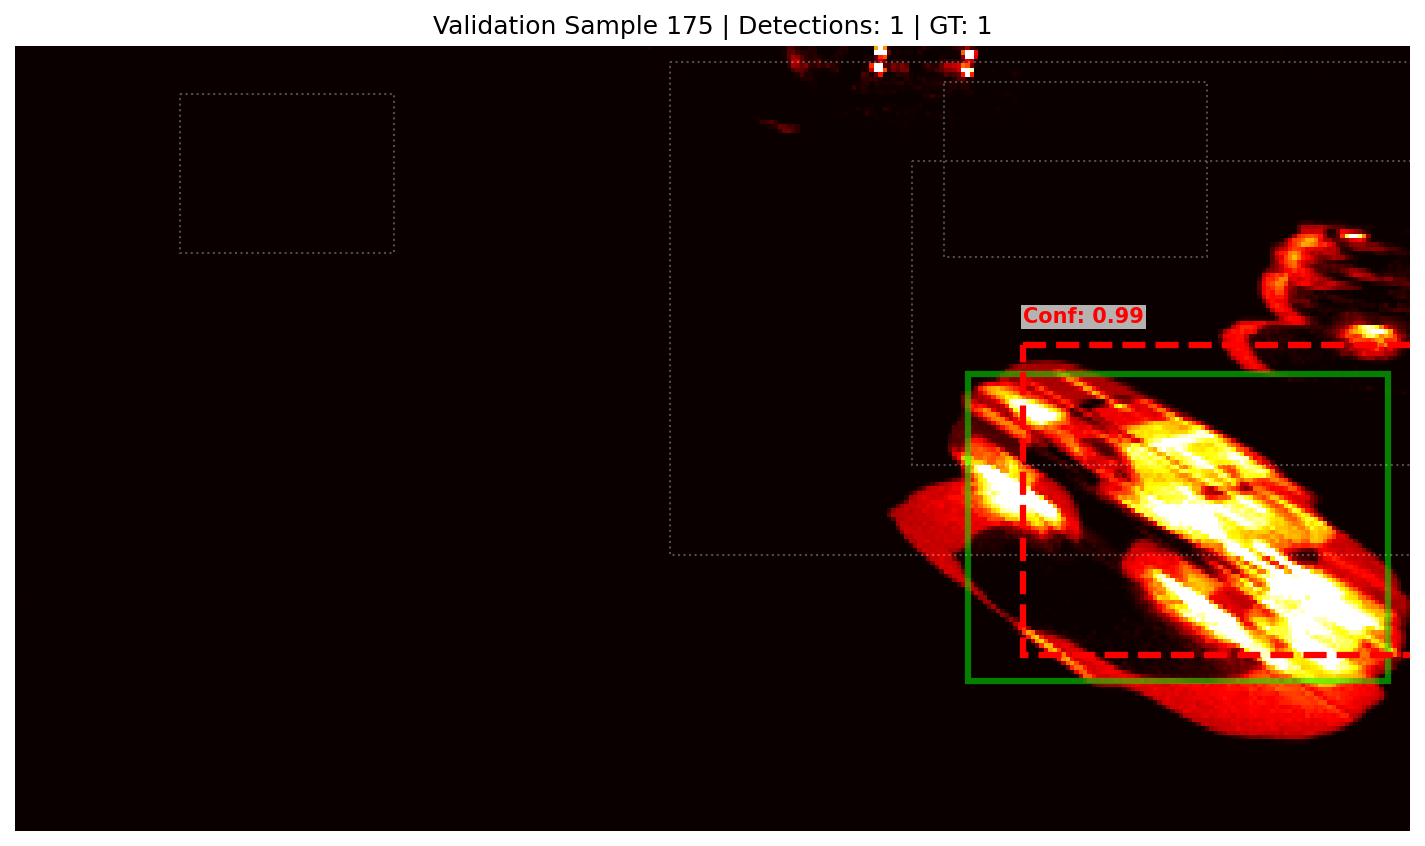
\includegraphics[width=0.45\textwidth]{chapter_3/dnx_results/cnn_audit/audit_sample_175.png} \\
\multicolumn{2}{@{}>{\centering\arraybackslash}p{0.92\textwidth}@{}}{\small\textit{Sample 175}} \\[0.5em]

\includegraphics[width=0.45\textwidth]{chapter_3/dnx_results/snn_audit/audit_sample_195.png} & 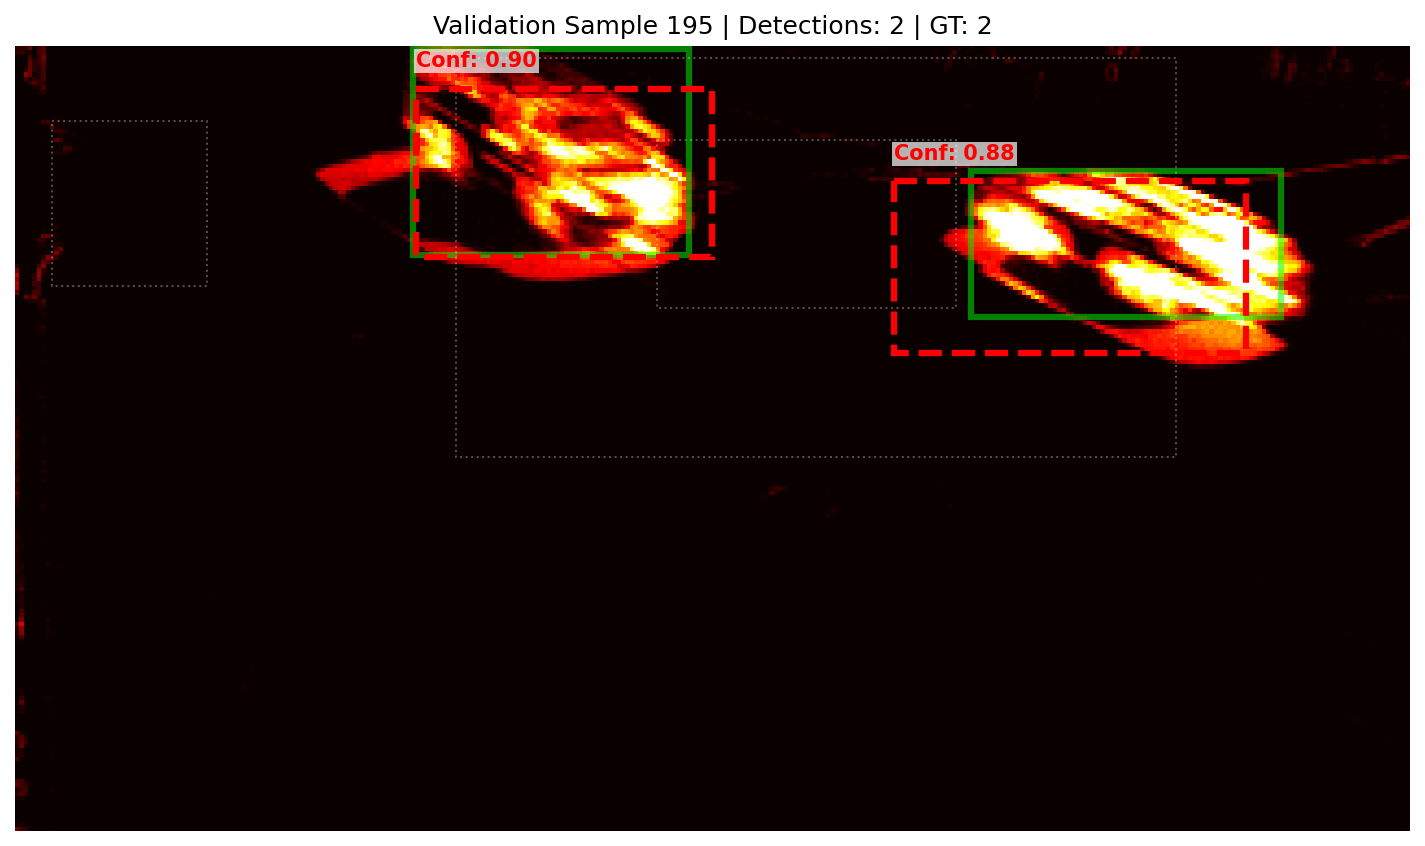
\includegraphics[width=0.45\textwidth]{chapter_3/dnx_results/cnn_audit/audit_sample_195.png} \\
\multicolumn{2}{@{}>{\centering\arraybackslash}p{0.92\textwidth}@{}}{\small\textit{Sample 195}} \\[0.5em]

% ============================================================
% 3. Dense Scenes (Three or More Objects)
% ============================================================
\multicolumn{2}{@{}l@{}}{\rule{0pt}{4ex}\textbf{\large 3. Dense Scenes (Three or More Objects)}} \\
\multicolumn{2}{@{}p{0.94\textwidth}@{}}{\itshape\small Higher-density frames stress-testing both architectures as object count rises. Sample 125 (four ground-truth vehicles) is the strongest density-handling case in the validation set.} \\
\hline

\includegraphics[width=0.45\textwidth]{chapter_3/dnx_results/snn_audit/audit_sample_095.png} & 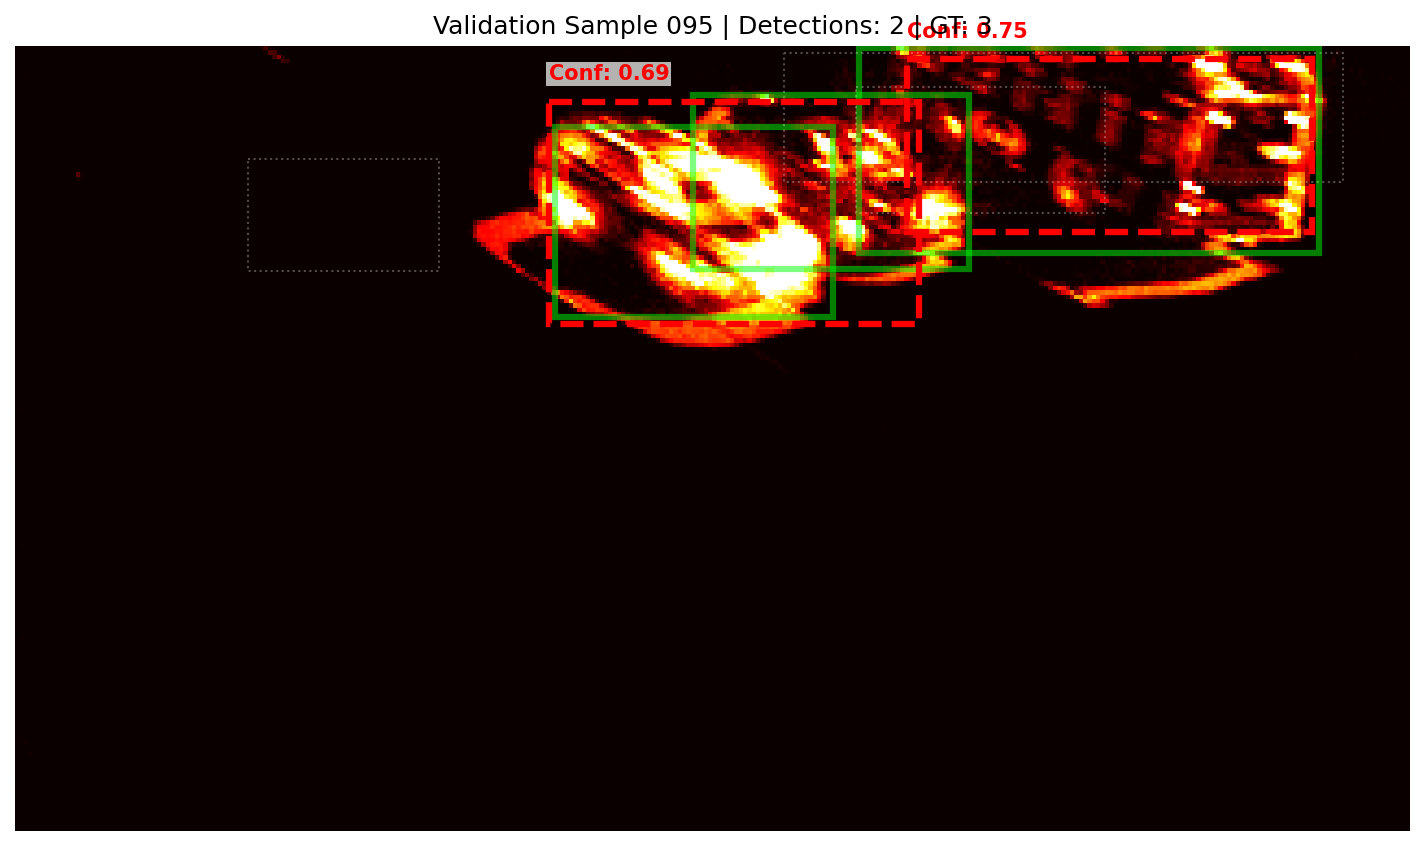
\includegraphics[width=0.45\textwidth]{chapter_3/dnx_results/cnn_audit/audit_sample_095.png} \\
\multicolumn{2}{@{}>{\centering\arraybackslash}p{0.92\textwidth}@{}}{\small\textit{Sample 095}} \\[0.5em]

\includegraphics[width=0.45\textwidth]{chapter_3/dnx_results/snn_audit/audit_sample_125.png} & 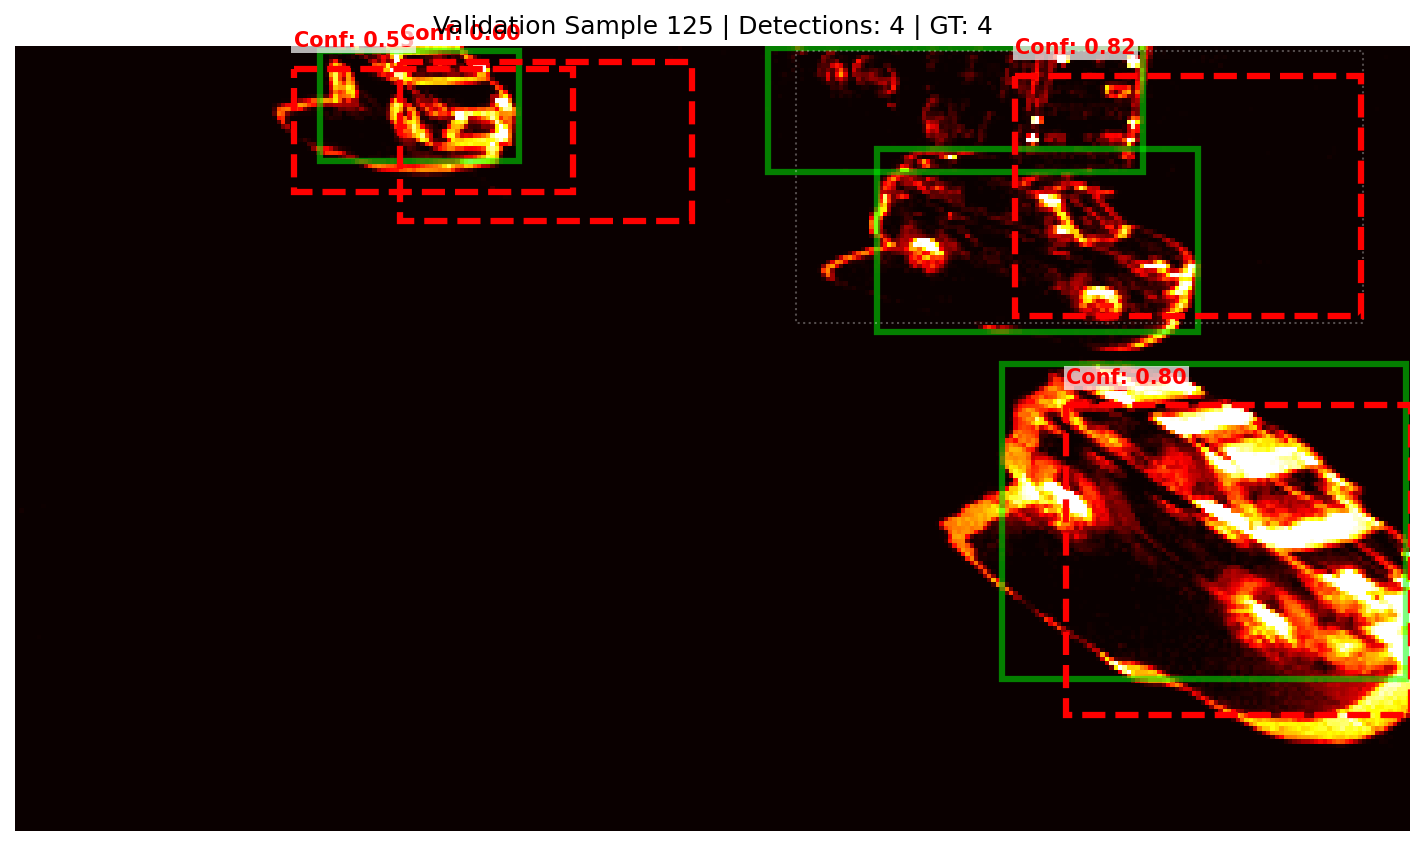
\includegraphics[width=0.45\textwidth]{chapter_3/dnx_results/cnn_audit/audit_sample_125.png} \\
\multicolumn{2}{@{}>{\centering\arraybackslash}p{0.92\textwidth}@{}}{\small\textit{Sample 125}} \\[0.5em]

% ============================================================
% 4. Architectural Divergence
% ============================================================
\multicolumn{2}{@{}l@{}}{\rule{0pt}{4ex}\textbf{\large 4. Architectural Divergence — Each Model Stronger on One Scene}} \\
\multicolumn{2}{@{}p{0.94\textwidth}@{}}{\itshape\small One scene where the SNN finds a vehicle the CNN misses, and one in the opposite direction. Both error directions exist; included to avoid one-sided framing.} \\
\hline

\includegraphics[width=0.45\textwidth]{chapter_3/dnx_results/snn_audit/audit_sample_155.png} & 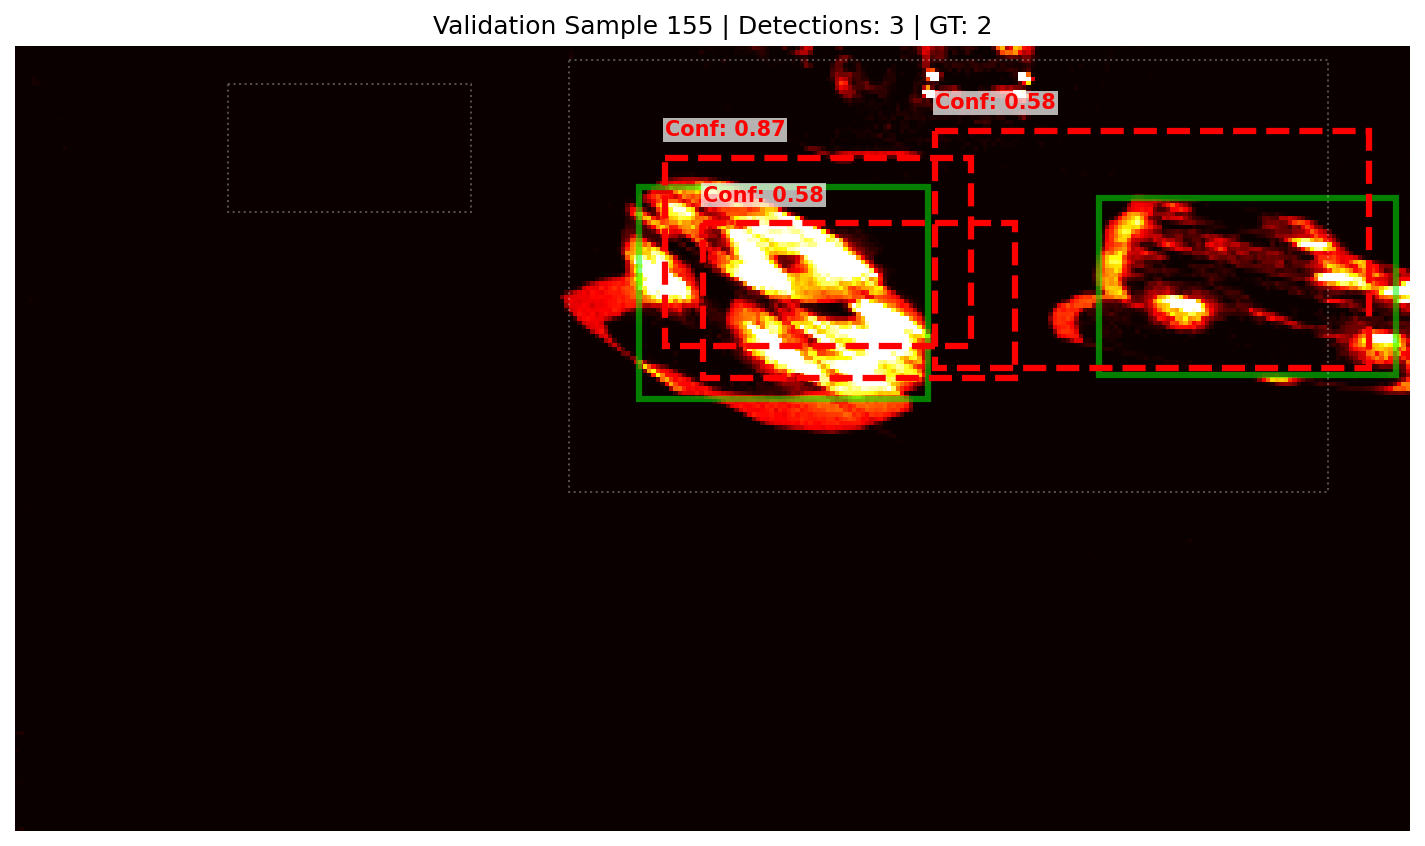
\includegraphics[width=0.45\textwidth]{chapter_3/dnx_results/cnn_audit/audit_sample_155.png} \\
\multicolumn{2}{@{}>{\centering\arraybackslash}p{0.92\textwidth}@{}}{\small\textit{Sample 155 — SNN detects both objects; CNN misses one.}} \\[0.5em]

\includegraphics[width=0.45\textwidth]{chapter_3/dnx_results/snn_audit/audit_sample_035.png} & 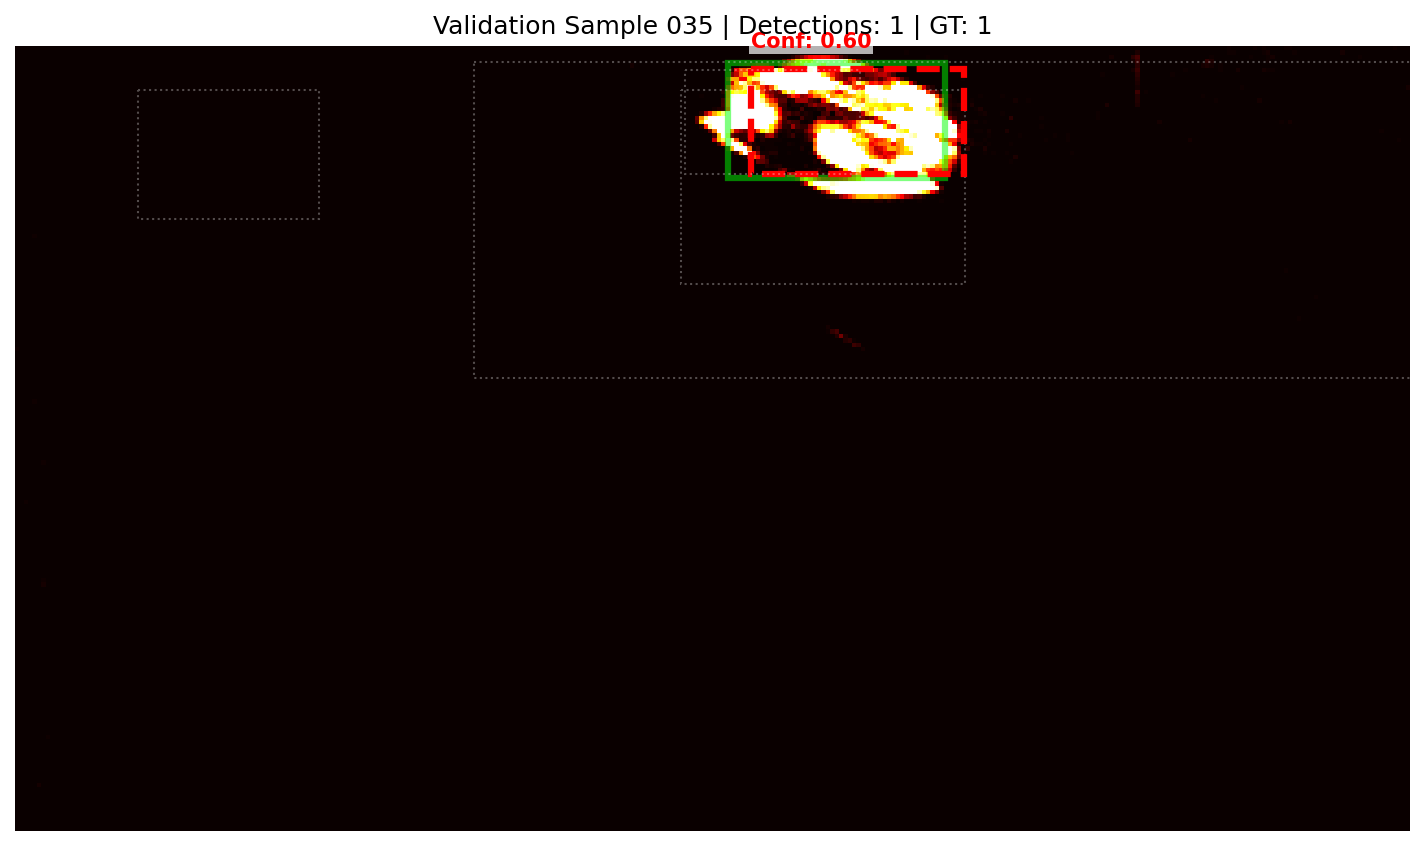
\includegraphics[width=0.45\textwidth]{chapter_3/dnx_results/cnn_audit/audit_sample_035.png} \\
\multicolumn{2}{@{}>{\centering\arraybackslash}p{0.92\textwidth}@{}}{\small\textit{Sample 035 — CNN detects the GT object; SNN misses it entirely.}} \\[0.5em]

% ============================================================
% 5. Divergent Counts (Over- and Under-Counting)
% ============================================================
\multicolumn{2}{@{}l@{}}{\rule{0pt}{4ex}\textbf{\large 5. Divergent Counts — Over- and Under-Counting}} \\
\multicolumn{2}{@{}p{0.94\textwidth}@{}}{\itshape\small Scenes where the two models disagree on the number of detections. Over-counting is not unique to either architecture.} \\
\hline

\includegraphics[width=0.45\textwidth]{chapter_3/dnx_results/snn_audit/audit_sample_015.png} & 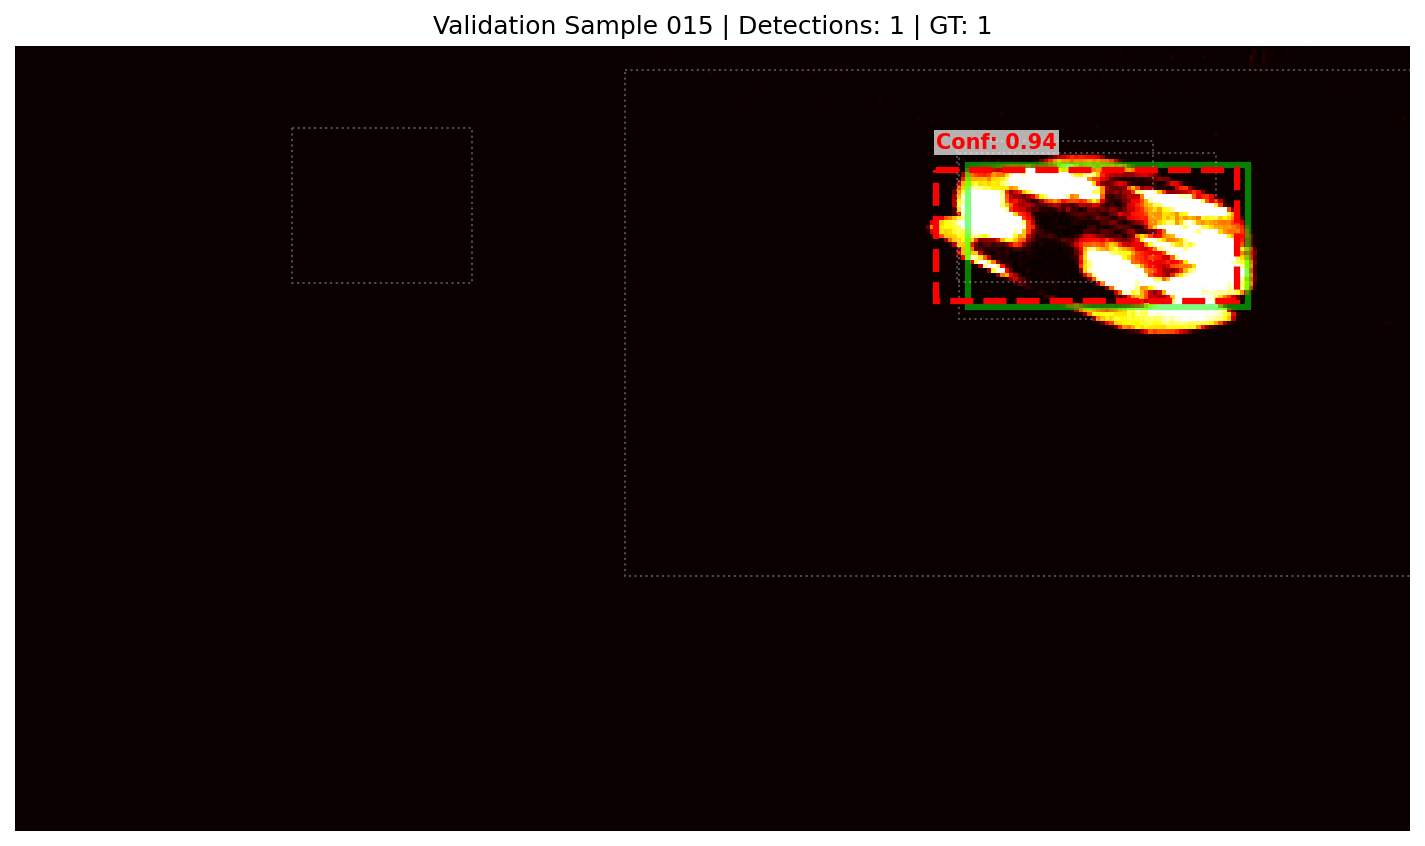
\includegraphics[width=0.45\textwidth]{chapter_3/dnx_results/cnn_audit/audit_sample_015.png} \\
\multicolumn{2}{@{}>{\centering\arraybackslash}p{0.92\textwidth}@{}}{\small\textit{Sample 015 — SNN reports two detections on a single-object scene; CNN clean.}} \\[0.5em]

\includegraphics[width=0.45\textwidth]{chapter_3/dnx_results/snn_audit/audit_sample_025.png} & 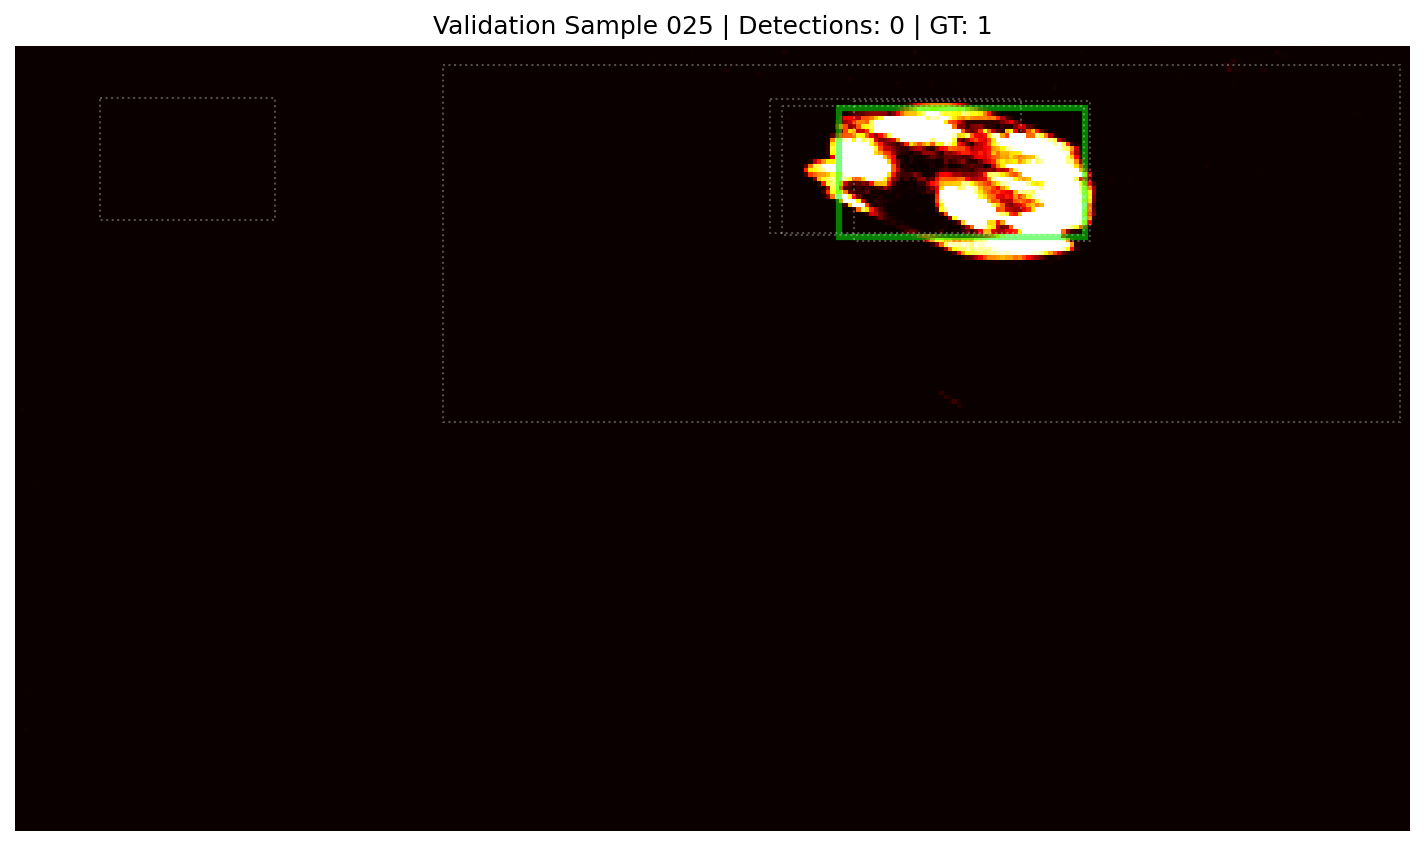
\includegraphics[width=0.45\textwidth]{chapter_3/dnx_results/cnn_audit/audit_sample_025.png} \\
\multicolumn{2}{@{}>{\centering\arraybackslash}p{0.92\textwidth}@{}}{\small\textit{Sample 025 — SNN over-counts; CNN misses entirely. Most divergent pair in the appendix.}} \\[0.5em]

\includegraphics[width=0.45\textwidth]{chapter_3/dnx_results/snn_audit/audit_sample_105.png} & 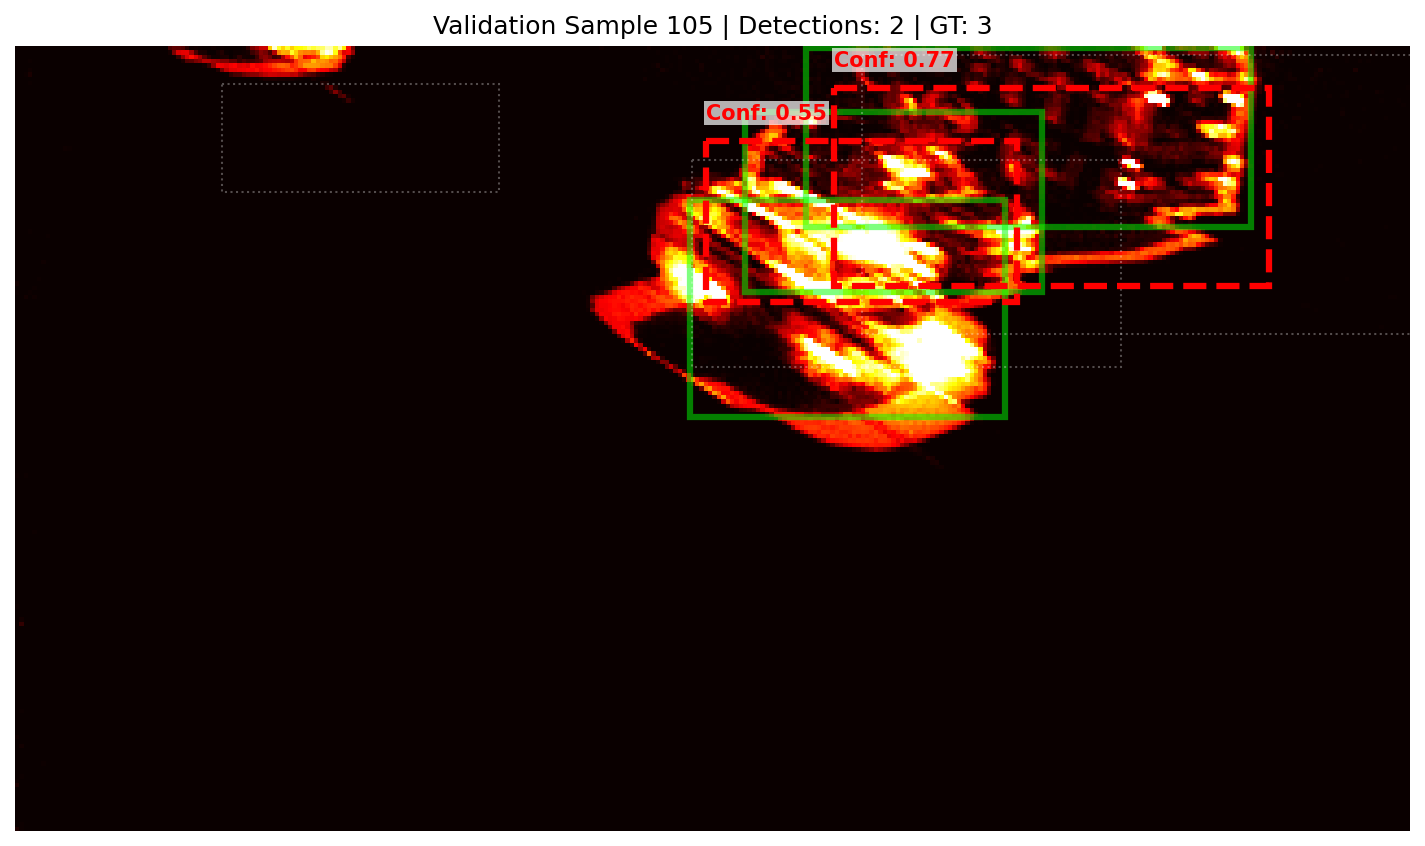
\includegraphics[width=0.45\textwidth]{chapter_3/dnx_results/cnn_audit/audit_sample_105.png} \\
\multicolumn{2}{@{}>{\centering\arraybackslash}p{0.92\textwidth}@{}}{\small\textit{Sample 105 — Mirror of 015: CNN over-counts; SNN clean.}} \\[0.5em]

% ============================================================
% 6. Calibration Evidence
% ============================================================
\multicolumn{2}{@{}l@{}}{\rule{0pt}{4ex}\textbf{\large 6. Calibration Evidence}} \\
\multicolumn{2}{@{}p{0.94\textwidth}@{}}{\itshape\small Cases reinforcing the implicit-uncertainty-sensor pattern characterised in Section~\ref{subsec:efficiency_landscape}: the SNN's confidence honestly tracks correctness, including dropping toward zero on ambiguous detections.} \\
\hline

\includegraphics[width=0.45\textwidth]{chapter_3/dnx_results/snn_audit/audit_sample_115.png} & 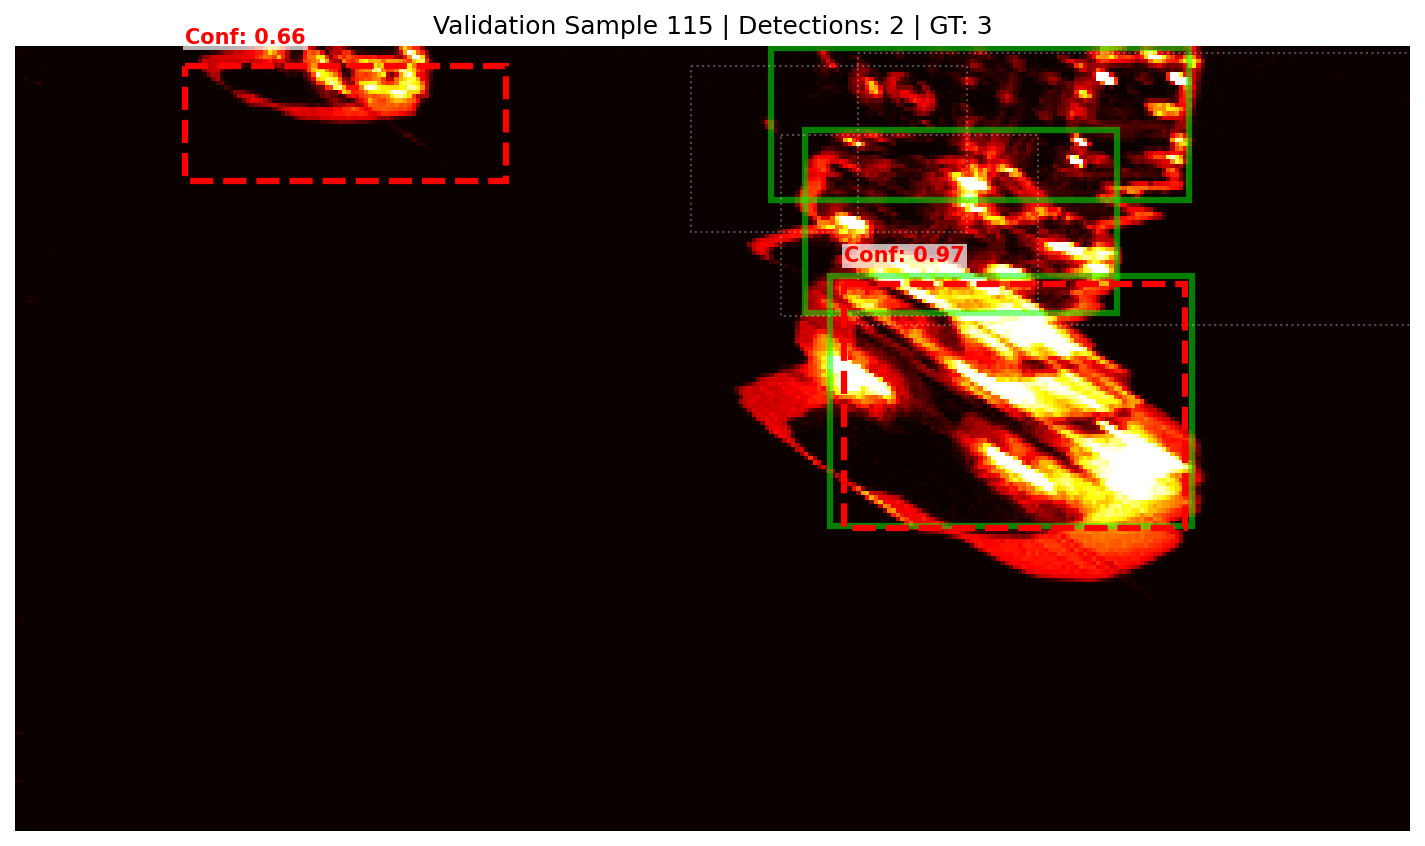
\includegraphics[width=0.45\textwidth]{chapter_3/dnx_results/cnn_audit/audit_sample_115.png} \\
\multicolumn{2}{@{}>{\centering\arraybackslash}p{0.92\textwidth}@{}}{\small\textit{Sample 115 — Confidence-vs-IoU divergence between the two architectures.}} \\[0.5em]

\includegraphics[width=0.45\textwidth]{chapter_3/dnx_results/snn_audit/audit_sample_135.png} & 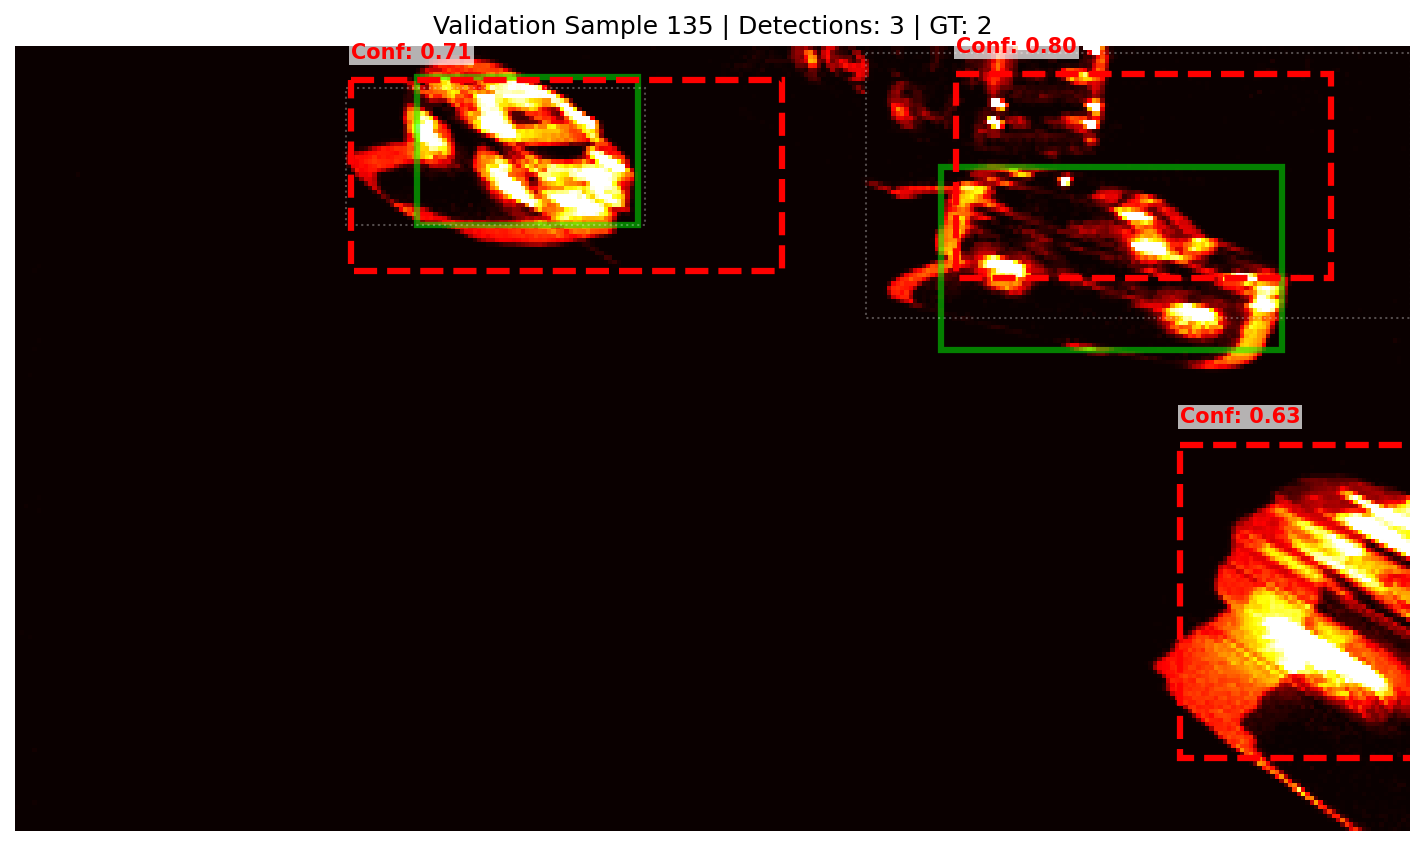
\includegraphics[width=0.45\textwidth]{chapter_3/dnx_results/cnn_audit/audit_sample_135.png} \\
\multicolumn{2}{@{}>{\centering\arraybackslash}p{0.92\textwidth}@{}}{\small\textit{Sample 135 — SNN reports a low-confidence detection ($\sim$0.41) on an ambiguous scene.}} \\[0.5em]

\includegraphics[width=0.45\textwidth]{chapter_3/dnx_results/snn_audit/audit_sample_185.png} & 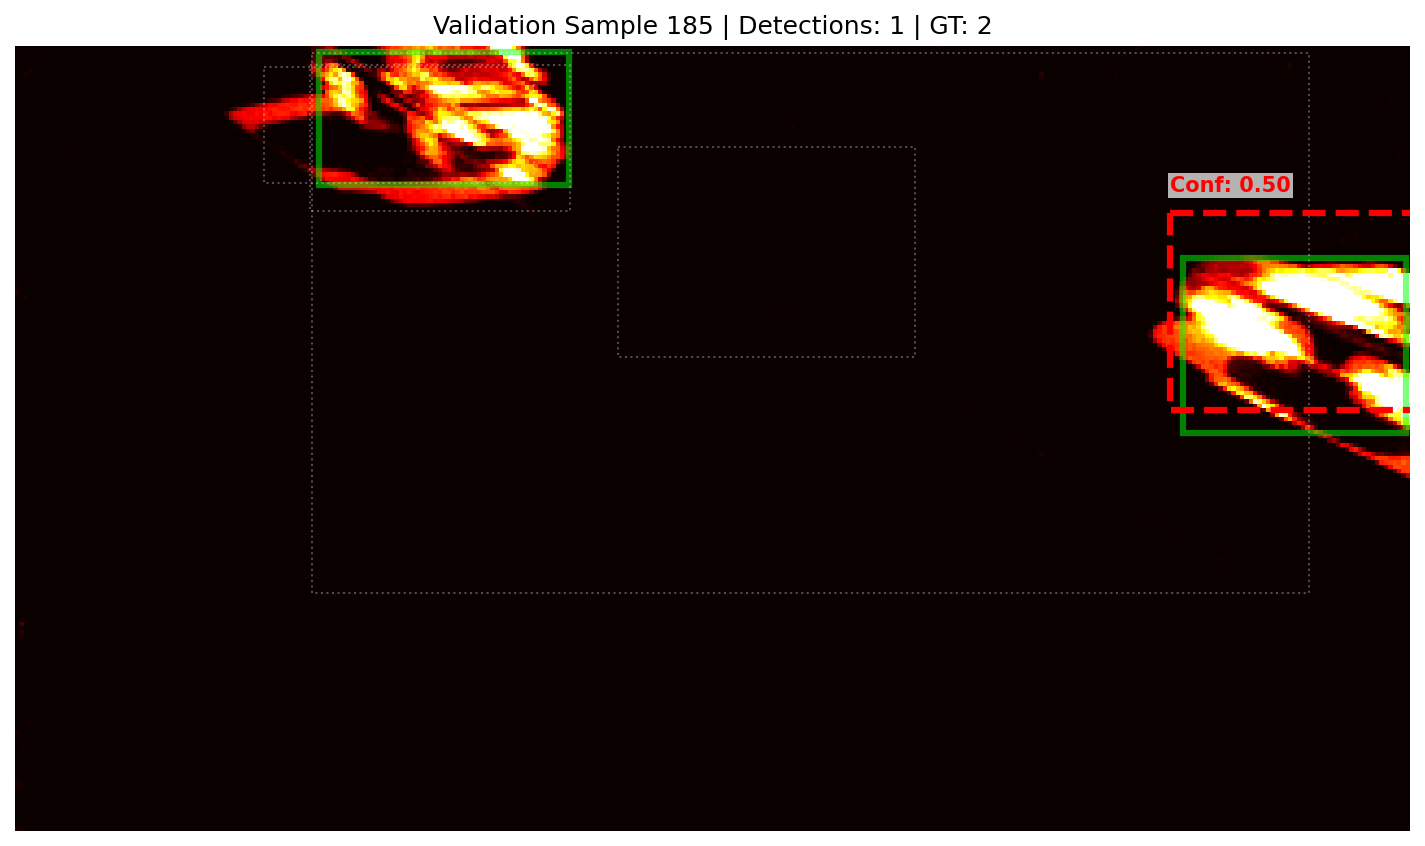
\includegraphics[width=0.45\textwidth]{chapter_3/dnx_results/cnn_audit/audit_sample_185.png} \\
\multicolumn{2}{@{}>{\centering\arraybackslash}p{0.92\textwidth}@{}}{\small\textit{Sample 185 — Very-low-confidence SNN prediction ($\sim$0.06) that nonetheless aligns with the GT box.}} \\[0.5em]

% ============================================================
% 7. Hard Scenes (Both Models Miss)
% ============================================================
\multicolumn{2}{@{}l@{}}{\rule{0pt}{4ex}\textbf{\large 7. Hard Scenes — Both Models Miss an Object}} \\
\multicolumn{2}{@{}p{0.94\textwidth}@{}}{\itshape\small Shared-failure scenes where both architectures drop one of the ground-truth vehicles. Honest acknowledgement of the validation set's harder cases.} \\
\hline

\includegraphics[width=0.45\textwidth]{chapter_3/dnx_results/snn_audit/audit_sample_085.png} & 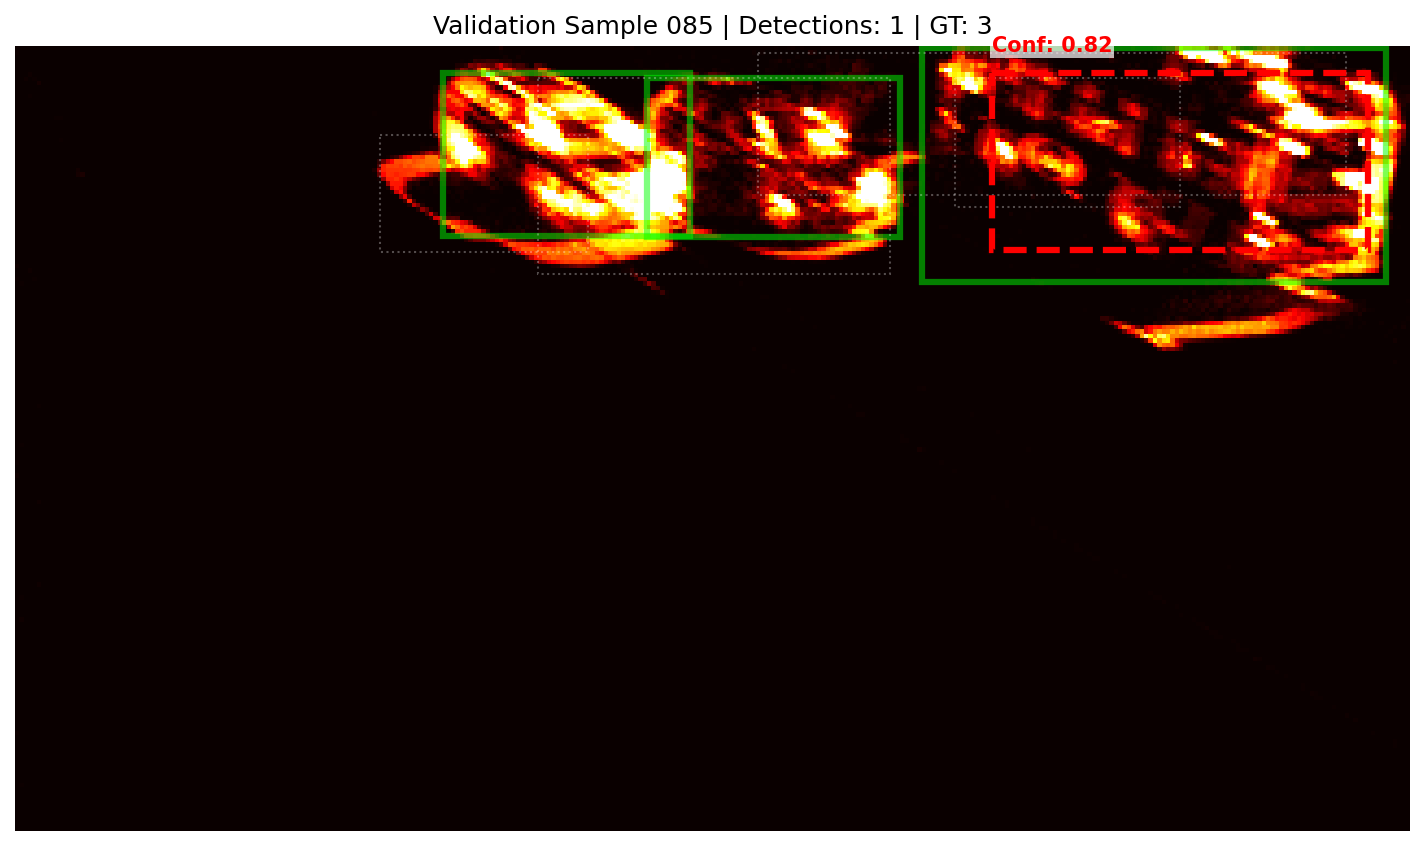
\includegraphics[width=0.45\textwidth]{chapter_3/dnx_results/cnn_audit/audit_sample_085.png} \\
\multicolumn{2}{@{}>{\centering\arraybackslash}p{0.92\textwidth}@{}}{\small\textit{Sample 085 — Both models report one of two ground-truth objects.}} \\[0.5em]

\includegraphics[width=0.45\textwidth]{chapter_3/dnx_results/snn_audit/audit_sample_165.png} & 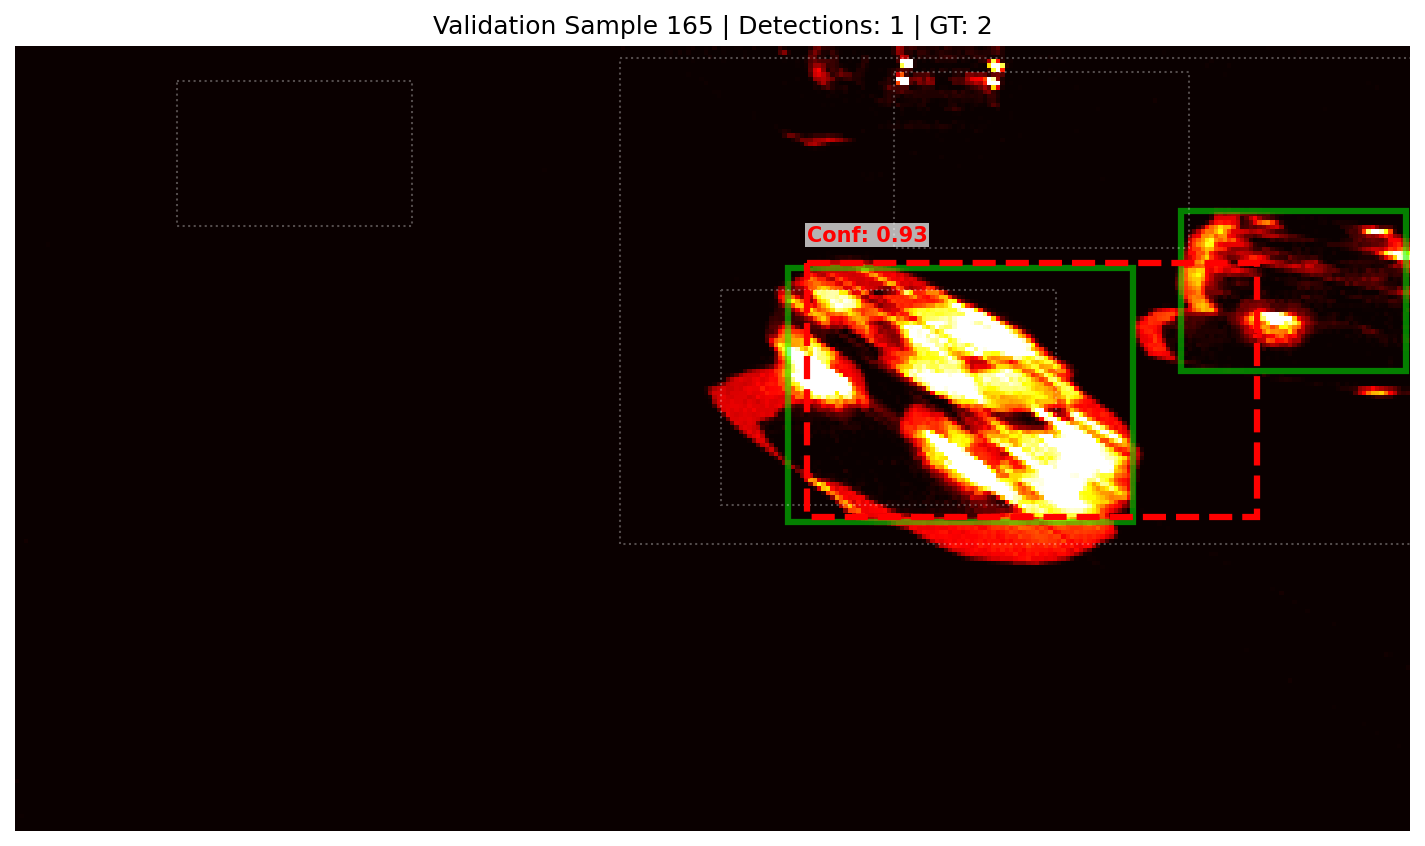
\includegraphics[width=0.45\textwidth]{chapter_3/dnx_results/cnn_audit/audit_sample_165.png} \\
\multicolumn{2}{@{}>{\centering\arraybackslash}p{0.92\textwidth}@{}}{\small\textit{Sample 165 — Same shared-miss pattern at a different validation-set point.}} \\[0.5em]
\end{longtable}

\vspace{1em}
\noindent\textbf{Full audit set.} The complete collection of 200 audit samples per model is available at the following link:

\begin{center}
\url{https://drive.google.com/drive/folders/1h6E90kFM59cgvdxO-J-FcohDKHsyNBEA?usp=sharing}
\end{center}
